\documentclass[a4paper,12pt]{article}
\usepackage[utf8]{inputenc}
\usepackage[top=2.5cm, bottom=2.5cm, left=2.5cm, right=2.5cm]{geometry}
\usepackage[english]{babel}
\usepackage{graphicx}
\usepackage{float}


% Title Page
\title{Université Libre de Bruxelles\\
INFO-F-404: Real-Time Operating Systems\\
2014 - 2015 Project 1: EDF}
\author{Picard Simon}
\date{December 12, 2014}

\begin{document}
\maketitle
\clearpage
\tableofcontents
\clearpage

\section{Introduction}
The purpose of the project is to implement an EDF scheduler which is a scheduler for multiprocessor operating system.\\
Three sub project were required, a tasks generator, the scheduler and a program that compare the result of the scheduler with different tasks propriety.

\section{Implementation}
\subsection{Tasks generator}
The first step is to divide the total utilization of the system by the number of tasks but some it is more interesting if the tasks do not have the same utilization so a normal distribution is used where the average is the total utilization divided by the number of process but it is not guaranteed that the sum of the utilization will be the total so some adjustment are then done.\\
Once the utilization for a task is set, the period is randomly generated between two values, the computing time of the tasks is the utilization percent times the period.\\
The deadline is a random number between the computing time and the period.\\
The offset is a random number between two given values.\\
Once all the tasks are generated some additional adjustment are done to be as close as possible to the utilization required.\\
Finally, the generated tasks are written in a file where each line describes one task and contains: Offset Period Deadline WCET.\\
Here is the options for the generator :
\begin{verbatim}
-o arg
    set the output file path
-u arg
    set the utilization of the resulting system
-n arg
    set the number of tasks
-p arg | default = 1
    set the floor for the period (this number wil be multiplicated by "Pfactor")
-P arg | default = 20
    set the roof for the period (this number wil be multiplicated by "Pfactor")
-x arg | default = 10
    set the roof for the "Pfactor"
-f arg | default = 0
    set the floor for the offset
-F arg | default = 10
    set the roof for the offset
-s
    generated a synchronous system, i.e no offset
-i
    generated implicit deadline, i.e deadline = period
\end{verbatim}

\subsection{EDF simulator}
The simulator begin by parsing the given tasks file description and create a Tasks object with the properties of the tasks.\\
The task object has a getNextJob function which returns the next jobs of the periodic task. The simulator generate the first job of each tasks then the simulator calculate the period of the system in order to simulated a full period system, this period is obtained by calculating the hyper period which is the least common multiple between all the tasks, increased by the biggest offset of the tasks.\\
Once the period is obtained, the simulator goes in loop which simulate one tick of the system, this loop is repeated for all the period. The simulator works with a list of job, one per tasks, first the simulator verify if any job are done, if it is, this job is discarded and the next job of the job's task is added to the list, then the release time of the jobs are set to the current system ticks if it is older. The jobs are then sorted by their release time and if some of them are equals, the one with the earliest deadline is placed before. The simulator verify that the deadline of the first job (and only this one because it is the one with the earliest) is exceed, if yes the tasks are not schedulable and the simulator stops else the simulator verify that it can execute a tick of the first job, if the release time of the first job is smaller of equal to the current system tick. If it is, the simulator verify it must calculate a switching time or a loading time and add it if it must, then execute a tick of the job and do this loop again.\\
Once all step are done, the simulator output the total period, the execution ticks, the idle ticks, the switching ticks and the number of preemptions.

\subsection{EDF study}
This part of the project is quite simple in its implementation, it has one main function genRun which given the properties for the tasks generation and the simulation will do both and return the output of the simulator.

\section{Difficulties meet}
The generation of the tasks was a bit complicated because the utilization must be as close as possible but the utilization of each tasks must not be the same so the solution was to use a uniform distribution and then adjust the total utilization, the adjustment will always output an utilization a bit lower than the required rather than a bigger one.\\
Another issue is that the system can have a really big period, so the period of the tasks are meant to be rather small and multiple of 10.\\
Finally, during the test I noticed that the tasks would often be not schedulable I therefore set the implicit option in place because it is not about a to big utilization but sometimes the jobs would just not possible to complete two would be released at the same time and have small deadline.

\section{Comparison tests}
There is several tests, the way they are done is explained in the Implementation section.\\
The first test is a schedulability test, with different utilization, number of tasks and switching time it is resulting which system is schedulable, this test id done with the default option.\\
The second one is the link between the period of the system and the number of tasks.\\
And three last are comparing all the outputs of the scheduler by varying the number of tasks, the utilization and the switching time.\\
The program create a file res.txt, in order to see the diagrams, the user must copy the content, open the file diagram.ods with Libre Office and past it in the top left cell of the file then hit the OK button in the dialogue, the diagrams are now updated with the new data.

\section{Study}
\subsection{Schedulability}
following different values for the utilization, the number of tasks and the switching time percent, the test simulate a hundred randomly generated system and give the number of schedulable one. See the figure down below for the result when varying the utilization.\\

\begin{figure}[H]
	\begin{center}
		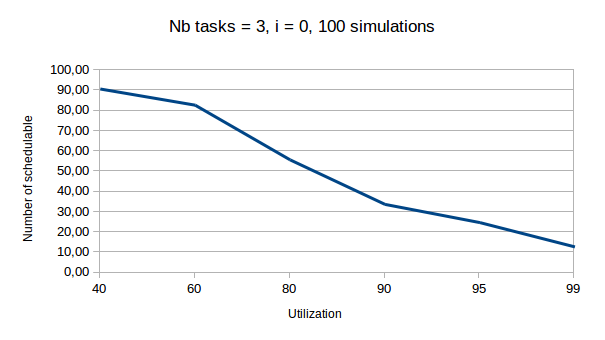
\includegraphics{schedU.png}
	\end{center}
	\label{sched}
	\caption{Schedulability over the utilization}
\end{figure}
It is clear that the more the utilization, the less the schedulabilty, the explaination is quite simple, the more utilisation the longer the utlisation of the tasks and therefore the bigger the chance to misse a deadline.

\begin{figure}[H]
	\begin{center}
		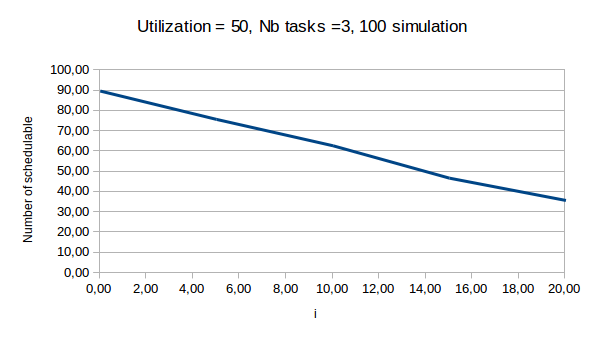
\includegraphics{schedI.png}
	\end{center}
	\label{sched}
	\caption{Schedulability over the switching percent}
\end{figure}

It appears that a big switching percent is the cause for a system to fail, the switching percent lead to the loss of some ticks and so a bigger probability for a job to miss it deadline.

\begin{figure}[H]
	\begin{center}
		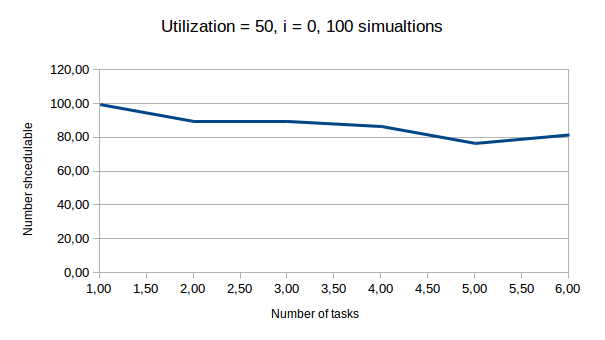
\includegraphics{schedN.png}
	\end{center}
	\label{sched}
	\caption{Schedulability over the number of tasks}
\end{figure}

The result is ambiguous, id there a lot a tasks the jobs will have a small utilisation, they will be loaded and executed rather fast so less chance of preemptions and missing the deadlines, but the more the tasks, the more the chance for two jobs with small deadlines to be realease at the same and miss their deadlines. These two effect are antagonist.

\subsection{Period}
The period depends on two factor, the offset and the period, it is the least common multiple of all the period plus the biggest offset, so it is LCM(P)+max(o) which is in O(LCM(P)), see the next figure for a graphic of the period in function of the number of tasks.\\

\begin{figure}[H]
	\begin{center}
		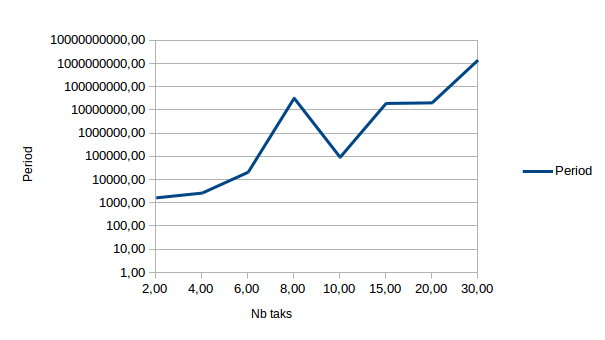
\includegraphics{periodtasks.png}
	\end{center}
	\label{period}
	\caption{Period}
\end{figure}
As expected, the period rise extremely fast following the number of tasks.

\subsection{Remark}
For this test and all the following, the generated tasks systems are synchronized and with implicit deadlines. Synchronized to have correct executing and idle time, otherwise all the first part of the system where all offset are not complete, the utilization of the system is not the one required. Implicit because, as we saw on the schedulability test, lots of system would fail just because the deadline are to small, it is almost impossible to complete a 99\% utilization system with deadlines that are not implicit.

\subsection{Utilization}
The two first test  are pretty obvious, it can be noticed that the number of tasks does not affect the utilization and that the execution time and the idle time are complementary.
\begin{figure}[H]
	\begin{center}
		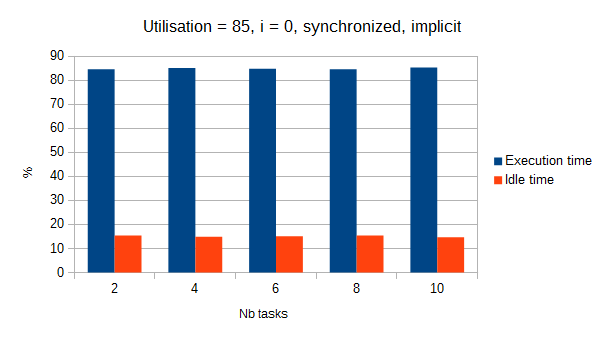
\includegraphics[scale=0.49]{nbtaskstime.png}
		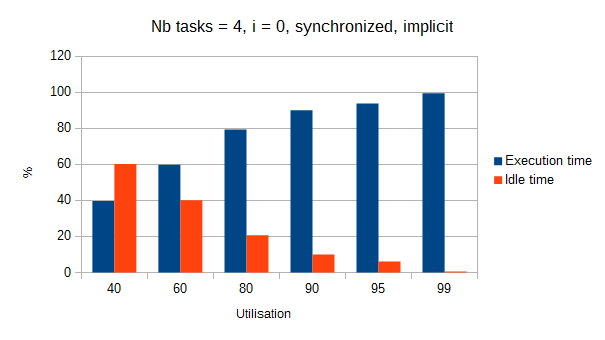
\includegraphics[scale=0.49]{utilisationtime.png}
	\end{center}
	\label{u}
	\caption{Utilization}
\end{figure}

Now with the same tasks system, this test compare the utilization with different switching time :
\begin{figure}[H]
	\begin{center}
		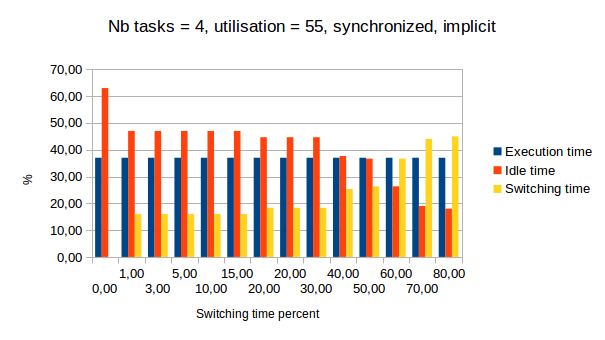
\includegraphics[scale=1]{switchingtime.png}
	\end{center}
	\label{us}
	\caption{Utilization over switching time}
\end{figure}

Firstly, the test has some plateau, this come from the rounding of switching time and from the small size of the number of computing ticks from the job. The execution time always takes the same part of the simulation, what change is idle time and switching. For 60\% of switching time and over, the system is not schedulable, this fail can be explained by two reasons, either there would more than 100\% of the total utilization of the system, that the idle could not compensate the switching time, or that the switching time of a job will make it miss it deadline even though there is still some idle time.

\subsection{Preemption}
\begin{figure}[H]
	\begin{center}
		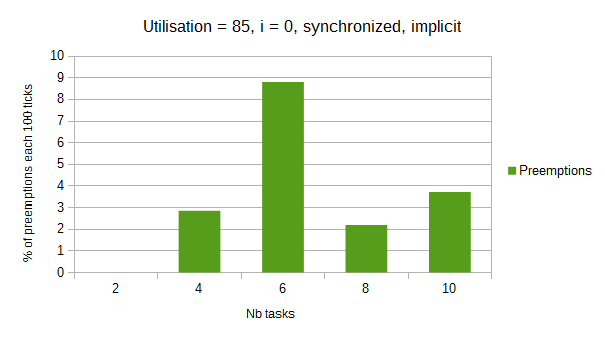
\includegraphics[scale=0.49]{nbtaskspreemption.png}
		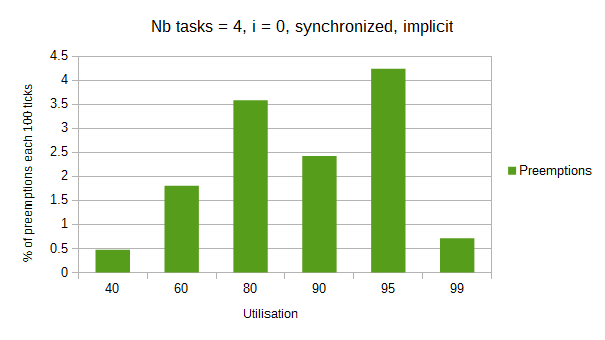
\includegraphics[scale=0.49]{utilisationpreemption.png}
	\end{center}
	\label{p}
	\caption{Preemptions}
\end{figure}

These tests do not make anything appear, there is apparently no correlation between the utilization or the number of tasks and the number of preemption.

\begin{figure}[H]
	\begin{center}
		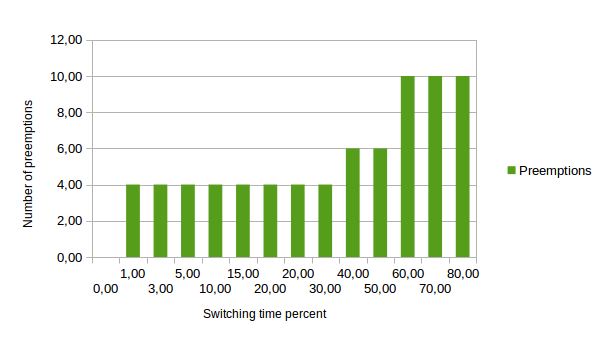
\includegraphics[scale=1]{switchingpreemption.png}
	\end{center}
	\label{p}
	\caption{Preemptions}
\end{figure}

Here, it is noticeable that the more the switching time the more preemption, this makes sense because after some switching a new job with an earlier deadline might be added to the jobs.


\end{document} 
